\section{Immobilization}
\begin{frame}
\subsubsection{Experiment Setup}
\frametitle{Vision-based 1-DOF Control}
\begin{columns}[c]
	\begin{column}{0.6\textwidth}
		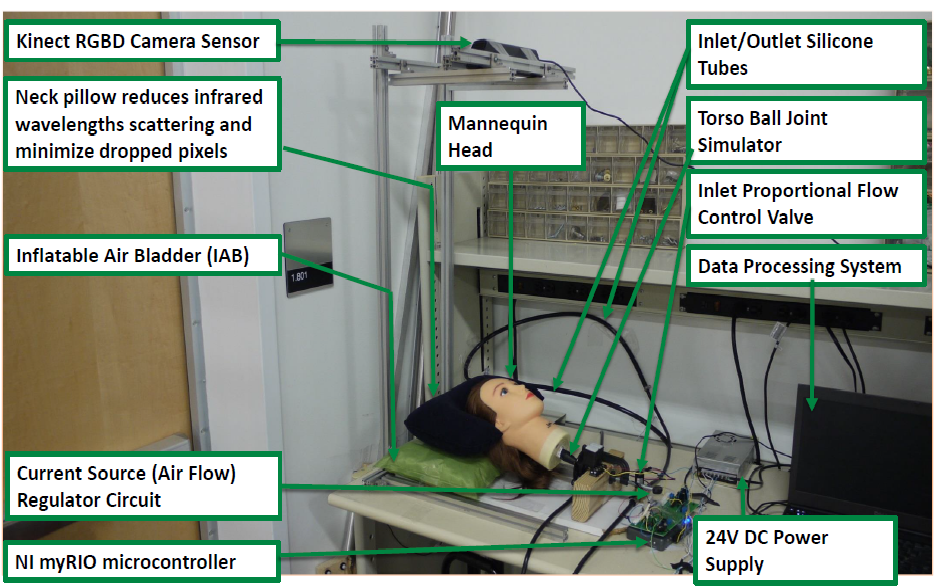
\includegraphics[width=\linewidth,height=.8\linewidth]{figures/setup_1dof.png}
	\end{column}
	%
	\begin{column}{0.48\linewidth}
		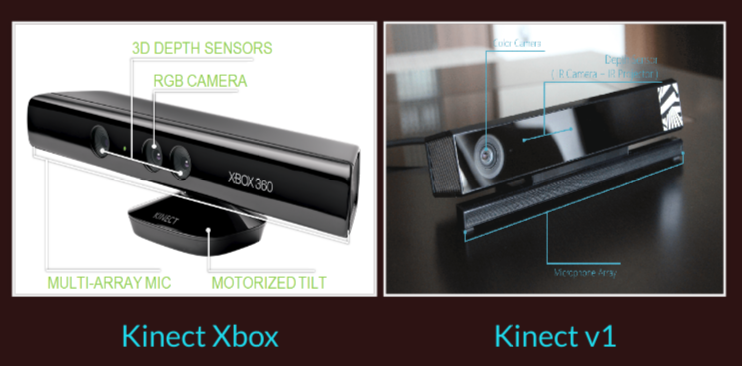
\includegraphics[width=\linewidth]{figures/kinects.png}
	\end{column}
\end{columns}
\end{frame}
%

\begin{frame}
\frametitle{Sensors' Noise Floor}
		\includegraphics[width=\columnwidth]{../../../SoftRobot/CASE2016/Charts/RawDepths.eps}
		%\centering Case for Sensed Observation Filtering
\end{frame}

\begin{frame}
\frametitle{Kalman Filter Model}
		\begin{align}
				\textbf{x}(k) &= \textbf{F}(k)\textbf{x}({k-1})+\textbf{B}(k)\textbf{u}_k+\textbf{G}_k\textbf{w}_k \nonumber \\
				%				
				\vspace{0.1in}
				%
				{z}_s &= \textbf{H}_s(k)\textbf{x}(k)+{v}_s(k) \qquad \qquad s = 1,2 \nonumber \\
				%				
				\vspace{0.1in}
				%
				\textbf{F} &= \begin{bmatrix}
									1 & \Delta T \\
									0	& 1
								\end{bmatrix}; \,
		 a_k \sim \mc{N}(0,  \sigma_a); \, \textbf{G}_k = \textbf{I}_{2x2};  \nonumber \\
		 \textbf{w}(k) &\sim \mathcal{N}(0, \textbf{Q}(k)), \,\,
		\textbf{W}(k) = \left(\begin{array}{c}
		\frac{{\Delta T}^2}{2} \\ \Delta T
		\end{array}\right) \nonumber \\
		%				
		\vspace{0.1in}
		%
		\textbf{Q} &= \textbf{W}\textbf{W}^T{\sigma_a}^2
		= \begin{bmatrix}
		\dfrac{{\Delta T}^4}{4} &	\dfrac{{\Delta T}^3}{2} \\
		\dfrac{{\Delta T}^3}{2} & {\Delta T}^2
		\end{bmatrix}{\sigma_a}^2.
		\end{align}
\end{frame}

\begin{frame}
	\frametitle{State Estimates | Global Fusion of Local Tracks}
	\begin{itemize}
		%\tiny
		\item \textbf{Prediction:}
		\begin{align}
		\hat{\textbf{x}}_{k|k-1}&=\textbf{F}\hat{\textbf{x}}_{k-1|k-1} + \textbf{B}_k\textbf{u}_k  \nonumber \\ 
		\textbf{P}_{k|k-1}&=\textbf{F}_k\textbf{P}_{k-1|k-1}{\textbf{F}_k}^T + \textbf{Q}_k
		\end{align}
		%
		\item \textbf{Update:}
		\small
		\begin{align} 
		\textbf{K}(k) &=  \textbf{P}(k|k-1){ \textbf{H}(k)}^T{[ \textbf{H}(k) \textbf{P}(k|k-1){ \textbf{H}(k)}^T+ \textbf{R}(k)]}^{-1}
		\nonumber \\ 
		\hat{ \textbf{x}}(k|k) &=\hat{ \textbf{x}}(k|k-1) +  \textbf{K}(k) ( \textbf{z}(k) -  \textbf{H}(k) \hat{ \textbf{x}}(k|k-1)) %\tilde{y}_k  
		\nonumber \\ 
		\textbf{P}(k|k)&=( \textbf{I} -  \textbf{K}(k) \textbf{H}(k)) \textbf{P}(k|k-1)
		\end{align}	
		%
%		\item \textbf{Fusion:}
%		\begin{align}
%		\hat{\textbf{x}}(F)(k|k) &= \textbf{P}(F)(k|k)\sum\limits_{s=1}^{N}\left[{\textbf{P}(s)}^{-1}(k|k)\hat{\textbf{x}}(s)(k|k)\right] \nonumber \\
%		\text{where    } \textbf{P}(F)(k|k) &= \left[\sum\limits_{s=1}^{N} {\textbf{P}(s)}^{-1}(k|k)\right]^{-1}. \nonumber
%		\end{align}
	\end{itemize}
\end{frame}

\begin{frame}
	\frametitle{Filtering Results}
		\centering
		\includegraphics[width=.45\columnwidth, height=0.4\columnwidth]{../../../SoftRobot/CASE2016/Charts/KFXbox.eps}
		\includegraphics[ width=.45\columnwidth,height=0.4\columnwidth]{../../../SoftRobot/CASE2016/Charts/Kinect2KF.eps} \\
		 Xbox vs. Kinect v1
		%
		\begin{itemize}
			\small \item 	\textbf{Fusion:}
			\begin{align}
			\hat{\textbf{x}}(F)(k|k) &= \textbf{P}(F)(k|k)\sum\limits_{s=1}^{N}\left[{\textbf{P}(s)}^{-1}(k|k)\hat{\textbf{x}}(s)(k|k)\right] \nonumber %\\
%			\text{where    } \textbf{P}(F)(k|k) &= \left[\sum\limits_{s=1}^{N} {\textbf{P}(s)}^{-1}(k|k)\right]^{-1}. \nonumber
			\end{align}
		\end{itemize}
\end{frame}

\begin{frame}
\frametitle{Fusion Results}
	\centering
\includegraphics[width=\columnwidth]{../../../SoftRobot/CASE2016/Charts/fusion2.eps}
\small Fusion of local state estimates.
\end{frame}

\subsection{Identification}
\begin{frame}
	\frametitle{System Model and LQG Control}
	\begin{itemize}
		\item Obtain optimal model parameters from I/O data through, 
		\begin{align}
		G(t)= \arg \min_{\theta} \, {V_N(\theta, \phi_N)} \label{eq:ident1} 
		\end{align}
		%
		\item From \eqref{eq:ident1}, we obtained
		%
		\begin{align} \label{eq:statemodel} 	
		\textbf{x}(k+Ts) = \textbf{A} \textbf{x}(k) + \textbf{B} \textbf{u}(k) + \textbf{K} \textbf{e}(k) \nonumber \\
		\textbf{y}(k) = \textbf{C} \textbf{x}(k) + \textbf{D} \textbf{u}(k) + \textbf{e}(k)
		\end{align} 
		%			
		\item LQG cost:
		\begin{equation}  \label{eqn:LQ-cost}
		J = \sum\limits_{k=0}^{\mathcal{K}} x^T(k)\,Q\,x(k) +  u(k)^T \, R \, u(k) + 2 x(k)^T \, N \, u(k) \nonumber
		\end{equation}  
		\item Find $u$ from $\Delta u  = \text{arg } \underset{\Delta u}{\text{min }}J $
		%\item  $\Delta{u}$ is a future control sequence
	\end{itemize}
\end{frame}

%\begin{frame}
%	\frametitle{Closed-loop control (Full state observer).}
%		\centering
%	\begin{tikzpicture}[thick,scale=0.4, every node/.style={transform shape}]
%	\sbEntree{E}
%	\sbBloc[4]{bloc1}{$\textbf{B}(k)$}{E}
%	\sbRelier[$\textbf{u}(k)$]{E}{bloc1}
%	\sbBloc[-2.7]{controller}{$\textbf{K}_{opt}$}{E}
%	
%	\sbSortie[-8]{starto}{controller}
%	\sbRelier{starto}{controller}
%	\sbNomLien[0.8]{starto-controller}{$\hat{\textbf{y}}(k)$}
%	
%	\sbCompSum[5]{sumbloc}{bloc1}{+}{+}{+}{}
%	\sbRelier{bloc1}{sumbloc}
%	\sbBloc[4]{integral}{$\int$}{sumbloc}	
%	\sbRelier{sumbloc}{integral}
%	\sbBloc[4]{Hprime}{$C(k)$}{integral}
%	\sbRelier[$x(k)$]{integral}{Hprime}
%	\sbCompSum[4]{sumtwobloc}{Hprime}{+}{}{+}{}
%	\sbRelier{Hprime}{sumtwobloc}
%	\sbDecaleNoeudy[-4]{sumbloc}{u}
%	\sbDecaleNoeudy{integral}{v}
%	\sbBlocr{F}{$A(k)$}{v}
%	\sbRelieryx{integral-Hprime}{F}
%	\sbRelierxy{F}{sumbloc}
%	\sbRelier{u}{sumbloc}   	
%	\sbNomLien[0.5]{u}{$w(k)$}
%	
%	\sbSortie[4]{y}{sumtwobloc}
%	\sbRelier{sumtwobloc}{y}
%	\sbNomLien[0.8]{y}{$y(k)$}
%	
%	\sbDecaleNoeudy[-4]{sumtwobloc}{w}	
%	\sbRelier{w}{sumtwobloc}
%	\sbNomLien[0.5]{w}{$v(k)$}
%	
%	\sbDecaleNoeudy{sumtwobloc-y}{v2}
%	\sbCompSum[8]{sum3bloc}{v2}{-}{+}{}{}
%	\sbRelierxy{y}{sum3bloc}
%	% % Estimator circuit
%	\sbDecaleNoeudy[9]{bloc1}{Ge}
%	\sbDecaleNoeudy[9.5]{Ge}{Gee}
%	\sbBlocr[-2]{Ghat}{$B(k)$}{Gee}
%	
%	\sbSortie[2]{GhatGee}{E}
%	\sbRelieryx{GhatGee}{Ghat}
%	
%	%\sbRelierxy{E}{Ghat}
%	\sbCompSum[7]{sume1}{Ghat}{+}{+}{+}{}
%	\sbRelier{Ghat}{sume1}
%	\sbBloc[4]{integrale}{$\int$}{sume1}	
%	\sbRelier{sume1}{integrale}
%	\sbBloc[4]{Hprimee}{$C(k)$}{integrale}
%	\sbRelier{integrale}{Hprimee}
%	%	\sbNomLien[3]{Hprimee}{$\hat{y}(k)$}
%	
%	\sbRelierxy[$\hat{y}(k)$]{Hprimee}{sum3bloc}
%	\sbDecaleNoeudy[-4]{sume1}{ue}
%	\sbDecaleNoeudy{integrale}{ve}
%	\sbBlocr{Fe}{$A(k)$}{ve}
%	\sbRelieryx{integrale-Hprimee}{Fe}
%	\sbRelierxy{Fe}{sume1}	
%	%  	\sbNomLien[0.5]{u}{$v(k)$}
%	\sbDecaleNoeudy[9]{sum3bloc}{xe}
%	\sbDecaleNoeudy[11]{xe}{xee}
%	
%	\sbDecaleNoeudy[-5.8]{sume1}{Ke}
%	\sbBloc[-1.5]{sume1}{-$K_{obs}$}{Ke}
%	\sbDecaleNoeudy{Ke}{sumpt}
%	\sbRelier{sume1}{sumpt}
%	
%	\sbSortie[-10]{arr}{sum3bloc}
%	\sbRelier[$\epsilon = \hat{y}(k) - y(k)$]{sum3bloc}{arr}  	
%	%\sbLien{sum3bloc}{arr} 
%	\sbDecaleNoeudy[9.5]{sumbloc-integral}{wL}
%	\sbSortie[-0.5]{wLL}{wL}	
%	\sbRelieryx{arr}{wLL}    
%	\sbSortie[-1.5]{Ltop}{sume1}
%	\sbDecaleNoeudy[-1.2]{Ltop}{Ltopey}
%	\sbRelier{wLL}{Ltopey}
%	%\sbNomLien[0.5]{w}{$w(k)$}
%	
%	\sbSortie[3]{we}{integrale} 
%	\sbRelieryx{we}{xee}
%	\sbNomLien[1]{xee}{$\hat{x}(k)$}
%	%\frame{
%	\frametitle{Control Design Goals}
%	\begin{columns}[c]
%		\begin{column}{\textwidth}
%			\begin{itemize}
%				\begin{itemize}
%					\item changing head shapes, size and other anatomic/tumor variations
%				\end{itemize}	
%			\end{itemize}
%		\centering
%		\includegraphics[width=0.95\linewidth,right]{../../IROS2017/Google/figures/mras.jpg}
%		\footnotesize Indirect MRAC system. \tiny (Source mdpi.com)
%			%
%		\end{column}
%		%
%	\end{columns}
%}
%	\sbDecaleNoeudy[3]{xee}{xeebutt}
%	\sbRelier{xee}{xeebutt}
%	\sbDecaleNoeudy[4.2]{Fe}{Ae}
%	\sbBlocr{ngtv}{$-1$}{Ae}
%	\sbRelier{xeebutt}{ngtv}
%	\sbRelierxy{ngtv}{controller}
%	
%	%\sbRelierxy{xee}{controller}
%	%
%	\sbSortie[4]{y}{sumtwobloc}
%	\sbRelier{sumtwobloc}{y}
%	\sbNomLien[0.8]{y}{$y(k)$}    
%	\end{tikzpicture} \\
%	%\centering \small Full Linear Quadratic Gaussian Plant Estimator \\
%	%\small State estimate: 
%	\small $\hat{x}(k+1) = A(k)\hat{x}(k) - K_{obs}[C(k)\hat{x}(k)- y(k)] + B(k)u(k).$
%\end{frame}

\begin{frame}
	\frametitle{1-DOF Control Results}
	%
	\centering
	\includegraphics[width=\columnwidth]{../../../SoftRobot/CASE2016/Charts/LQGI.eps}
%	\includegraphics[width=0.45\columnwidth, height=0.4\columnwidth]{../../../SoftRobot/CASE2016/Charts/LQGIII.eps}
	\\
	\centering LQG Controller on mannequine head.
\end{frame}


\subsection{3-DOF Control}

\begin{frame}
\frametitle{Vision-based 3-DOF Control}
	\centering
	\includegraphics[width=\columnwidth]{../../../SoftRobot/IROS2017/figures/setup/testbed.jpg}
	\centering Hardware Description
\end{frame}
\frame{
	\frametitle{Point Cloud Pre-Processing}
	\begin{columns}[c]
		\begin{column}{0.95\textwidth}	
			\begin{figure}
				\begin{center}
					\includegraphics[width=.8\linewidth]{../../../SoftRobot/IROS2017/figures/seg_cloud_nice.jpg}			
				\end{center}
			\end{figure}
		\end{column}
		%
	\end{columns}
}

\frame{
	\frametitle{Head Pose Estimation}
	\begin{itemize}
		\item Set cloud's centroid as measured point set $\textbf{P} = \{\overrightarrow{p}_i\}$
		%
		\vspace{0.1in}
		%
		\item Get covariance matrix $\Sigma_{px}$ of measured and model point sets: $\textbf{P}$ and $\textbf{X}$
		%
		\vspace{0.1in}
		%
		\item Set cyclic components of anti-symmetric matrix as $\Delta$
		%
		\vspace{0.1in}
		%
		\item Set $\textbf{Q}(\bm{\Sigma}_{px}) = \begin{bmatrix}
		\textbf{tr}(\bm{\Sigma}_{px}) & \bm{\Delta}^T \\
		\bm{\Delta} & \bm{\Sigma}_{px} + \bm{\Sigma}_{px}^T - \textbf{tr}(\bm{\Sigma}_{px})\textbf{I}_3
		\end{bmatrix}$
		%
		\vspace{0.1in}
		%
		\item $q_R = \underset{\text{eig}}{\max} \left(\textbf{Q}(\bm{\Sigma}_{px})\right)$; $q_T = \mu_x - \textbf{R}(q_R)\mu_p$
		%
		\vspace{0.1in}
		%
		\item 	$x_h = (q_T, q_R)$ %Relative orientation and position of head and neck system \wrt table frame	
	\end{itemize}
}

\subsection{Adaptive NeuroControl}
\frame{
	\frametitle{Model Reference Adaptive Control}
	\begin{itemize}
		%
		\item Head and IAB System Model
		%
		\begin{align}
			\dot{\textbf{y}} = \textbf{A}\textbf{y} + \textbf{B} {\bm \Lambda} \left(\textbf{u} - f(\textbf{y}, \textbf{u}) \right) + \textbf{w}(k) \nonumber
		\end{align}
		 %
		 \item  Realize $f(\textbf{\textbf{y}, \textbf{u}})$ with an RNN $\equiv \Theta^T \Phi(\textbf{y})$ 
		 %
		 \vspace{0.1in}
		 %		
		 \item In a ball $\textbf{B}_R \subset D$ %where the domain $D$ in $\reline^n$ contains $f(\cdot)$:
		 %
		 \vspace{0.1in}
		 %		
		 \begin{itemize}
		 	\footnotesize \item an ideal neural network (NN) approximation $f(\cdot): \reline^n \rightarrow \reline^m$, can be realized to a sufficient degree of accuracy, $\varepsilon_f > 0$;
		 \end{itemize}
		 %
 		\vspace{0.1in}
		%				 
		 \item Outside $\textbf{B}_R$:
		 %
		 \vspace{0.1in}
		 %				 
		 \begin{itemize}
		 	\footnotesize \item %the NN approximation error is upper-bounded by a known scalar function $\varepsilon_{max}(\textbf{y})$ \ie
		 	 $\|\varepsilon(\textbf{y})\| \le k_{\text{max}}(\textbf{y}), \quad \, \forall \quad \textbf{y} \in \textbf{B}_R$;
		 \end{itemize}
	\end{itemize}		
}

\frame{
	\frametitle{Adaptive Neuro-Control Scheme}
	\begin{itemize}
		\item Choose $\dot{\textbf{y}}_m = \textbf{A}_m y_m + \textbf{B}_m \textbf{r}$ 
		%
		\vspace{0.1in}
		%
		\item Knowns: $B_m$ and an Hurwitz $A_m$%Adaptive adjustment mechanism from Lyapunov analysis (Parks, P., 1966)
		%
		\vspace{0.1in}
		%				
		\item $\textbf{u} = \underbrace{\hat{\textbf{K}}_y^{\textbf{T}}\textbf{y}}_{\text{state feedback}} + \underbrace{\hat{\textbf{K}}_r^{\textbf{T}} \textbf{r}}_{\text{optimal regulator}} + \underbrace{\hat{f}(\textbf{y, u})}_{\text{approximator}}$
		%
		\vspace{0.1in}
		%
		\item $\hat{\textbf{K}}_y \, \text{ and } \hat{\textbf{K}}_r$ are adaptive gains to be  designed. 
		NB:  $\tilde{\textbf{K}}_x = \textbf{K}_x - \hat{\textbf{K}}_x$
		%	
		\vspace{0.1in}
		%	
		\item Assume ideal model matching conditions $\hat{\textbf{K}}_y = \textbf{K}_y , \, \text{ and } \hat{\textbf{K}}_r = \textbf{K}_r$ 
	\end{itemize}
}

\frame{
	\frametitle{Lyapunov Analysis}
	%
	\begin{itemize}
		\small
		\item \textbf{Theorem:} Given correct choice of adaptive gains $\hat{\textbf{K}}_y$ and $\hat{\textbf{K}}_r$, the error state vector, $\textbf{e}(k)$ with closed loop time derivative $\dot{\textbf{e}}$, is \textit{\textbf{uniformly ultimately bounded}}, and the state $\textbf{y}$ will converge to a neighborhood of $\textbf{r}$ (proof in ~\cite[\S V.A]{Ogunmolu17IROS}).
		%
		\vspace{0.1in}
		%
		
		\item Choose 
					\begin{align}
					\textbf{V}(\textbf{e}, \tilde{\textbf{K}}_y, \tilde{\textbf{K}}_r^T) =
					%
					\textbf{e}^T\textbf{P}\textbf{e} 
					%
					+\textbf{tr}(\tilde{\textbf{K}}_y^T  \bm \Gamma_y ^{-1}  \tilde{\textbf{K}}_y^T |\bm \Lambda|) %\nonumber 
					+\textbf{tr}(\tilde{\textbf{K}}_r^T \Gamma_r^{-1} \tilde{\textbf{K}}_r |\bm \Lambda|) \nonumber
					\end{align}
		%
		\item Neural network model $\hat{f}(\textbf{y}) = \hat{{\bm \Theta}}^T {\bm \Phi}(\textbf{y}) + \bm \varepsilon_f(\textbf{y})$
	\end{itemize}
}

\frame{
	\frametitle{Proof Main Matter}
	%\begin{itemize}		
		%
		\begin{align}
		\lyapder(\textbf{e}, \tilde{\textbf{K}}_y, \tilde{\textbf{K}}_r^T) &= -\textbf{e}^T\textbf{Qe}  -2 \textbf{e}^T\textbf{PB}\lamb \neterror \nonumber \\
		\lyapder(\textbf{e}, \tilde{\textbf{K}}_y, \tilde{\textbf{K}}_r^T) & \le -\lambda_{low}\|\textbf{e}\|^2 + 2\|\xbold{e}\| \|\textbf{PB}\|\lambda_{high}(\lamb) \bm{\varepsilon}_{max} \nonumber 
		\end{align}
		
		\begin{tcolorbox}[title=Term Contributions,colframe=green!35!blue!75]
			\begin{itemize}
				\item  $\hat{\textbf{K}}_y^{\textbf{T}}\textbf{y} $  keeps  $\textbf{y} \in \textbf{B}_R$ stable; $\hat{\textbf{K}}_r^{\textbf{T}} \textbf{r}$ reference tracking
				%
				\item $\hat{f}(\textbf{y}, \control)$ ensures states starting outside  set $\textbf{y} \in \textbf{B}_R$ converge to $\textbf{B}_R$ in finite time 
			\end{itemize}
		\end{tcolorbox}	
	%\end{itemize}
}

\frame{
	\frametitle{Proof Main Matter}
	%
	\begin{itemize}
		\item $\lambda_{low}, \lambda_{high}$ $\equiv$ minimum and maximum characteristic roots of $Q \text{ and }\lamb$ respectively
		%
		\vspace{0.1in}
		%
		\item $\dot{\xbold{V}}(\cdot)$ is thus negative definite outside the compact set:
		%
		\vspace{0.1in}
		%
		\begin{itemize}
			\item $\chi =\left(\textbf{e}: \|\textbf{e}\| \le \frac{2\|\textbf{PB}\|\lambda_{high}(\bm \Lambda)\varepsilon_{max}(\textbf{y})}{\lambda_{low}(\textbf{Q})}\right)$
		\end{itemize}
		%
		\vspace{0.1in}
		%
		\item Therefore, the error $\textbf{e}$ is uniformly ultimately bounded $\textbf{y}(t) \rightarrow 0$ as $t \rightarrow \infty$
	\end{itemize}
}
\frame{
	\frametitle{Results}
	\begin{itemize}
				\item Choose
				\begin{align}
				\textbf{P} = 
				\begin{bmatrix}
				-\frac{170500}{2668} & 0 & 0 \\
				0 & -\frac{170500}{2668} & 0 \\
				0 & 0 & -\frac{170500}{2668}
				\end{bmatrix} \nonumber
				\end{align}			
				\item and set 	
				\begin{align}
					\textbf{B} = 
					\begin{bmatrix}
					1 &\, 1 &\, 0 &\, 0  &\, 0 &\, 0 \\
					0 &\,  0 &\, 1 &\, 1 &\, 0 &\, 0 \\
					0 &\,  0 &\, 0 &\, 0 &\,  1 &\, 1 
					\end{bmatrix} \nonumber
					\end{align}
			\end{itemize}
}

\frame{
	\frametitle{Results}
	%
		\centering
		\includegraphics[width=0.45\columnwidth,height=0.35\columnwidth]{../../IROS2017/Google/figures/expt2a.eps}
		\includegraphics[width=0.45\columnwidth,height=0.35\columnwidth]{../../IROS2017/Google/figures/roll_nice.eps}
		\footnotesize \centering 
		[Left]: Goal command: $\left(z, \theta, \phi\right)=\left(2.5mm, 0.25^\circ, 35^\circ\right)$ to $\left(14mm, 1.6^\circ, 45^\circ\right)^T$. 
		\centering[Right]: Head roll tracking.
}
